\chapter{Cache e RAM}

\textsc{Definição} \textbf{Princípio de Localidade:} programas tendem a reusar dados e instruções que foram usadas recentemente. Podemos dividir em:

\begin{itemize}
  \item \textbf{Localidade temporal:} itens acessados recentemente têm grande probabilidade de serem acessados novamente;

  \item \textbf{Localidade espacial:} itens cujos endereços estão próximos tendem a ser acessados em tempos próximos.
\end{itemize}

Logo temos a possibilidade de prever instruções que serão utilizadas em um futuro próximo com base em acessos recentes. Isso justifica o uso da \textbf{hierarquia de memória}.


\section{Cache}
\textsc{Definição} Memória rápida e com pouca capacidade de armazenamento. Interposta entre a CPU e a memória principal. A medida de dados é feita em \textbf{WORDS} (palavras), a qual normalmente trocada entre CPU e cache. Definimos:

\textbf{Cache hit:} o dado procurado está em cache

\textbf{Cache miss:} o dado procurado NÃO está em cache

\begin{figure}[ht]
  \centering
  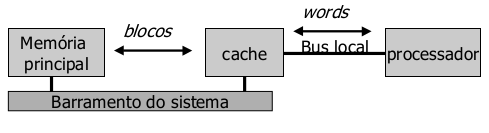
\includegraphics[width=0.8\textwidth]{cache-arch}
  \label{fig:cache-arc}
  \caption{Detalhes de ligação entre cache, processador e memória}
\end{figure}

\subsection{Colocações e Localização de Bloco em Cache}
A cache é bem menor que a memória, logo precisamos de um modo de inserir blocos da memória na cache e indexa-los de forma eficaz. O formato de um endereço do ponto de vista da \textit{cache} segue a Figura \ref{fig:address-cache}. Dentro de um endereço de tamanho $A$, temos:

\begin{figure}[ht]
  \centering
  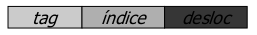
\includegraphics[width=0.6\textwidth]{cache-addr}
  \caption{Estrutura do endereço do dado, do ponto de vista da \textbf{cache}}
  \label{fig:address-cache}
\end{figure}

\begin{itemize}
  \item \textbf{Índice - $I$}: a posição do bloco dentro da cache. No caso do set associative, é o índice do conjunto em que o bloco se encontra.
  \begin{equation}
    I = \lg{\frac{C}{b}}
  \end{equation}

  \item \textbf{Deslocamento - D}: é índice da palavra em que o dado se encontra, em relação ao bloco. Deve ser o número de bits para representar o número de palavras em um bloco;
  \begin{equation}
    D = \lg{w}
  \end{equation}

  \item \textbf{Tag - T}: verificador usado para indicar se há um miss ou um hit na hora do acesso. É sempre o que sobra no endereço depois do índice e deslocamento.
  \begin{equation}
    T = A - (I + D)
  \end{equation}
\end{itemize}

A seguir, iremos definir como esse endereço se estrutura ao longo dos três tipos de colocação do bloco em cache. A Figura \ref{fig:cache-placement} dá um ótimo exemplo de como um mesmo dado é colocado e disponibilizado ao longo dos três métodos. Antes, defina que a cache tem tamanho $C$, com blocos de tamanho $B = w.b$, onde $w$ é o tamanho da palavra e $b$ o número de bytes por palavra. Para sabermos o número total de blocos $N_B$ dentro da cache, usaremos a Equação \ref{eq:cache-blocks}.

\begin{equation}
N_B = \frac{C}{b}
\label{eq:cache-blocks}
\end{equation}

\begin{figure}[ht]
  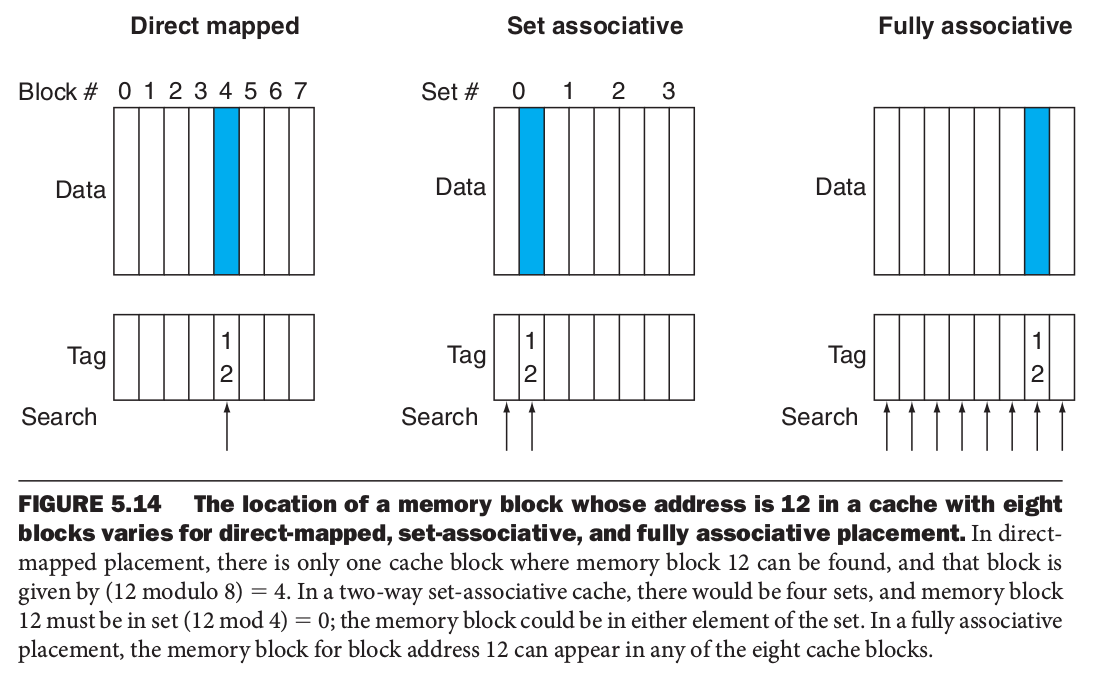
\includegraphics[width=\textwidth]{cache-placement}
  \caption{Diferentes abordagens para colocação de cache. Desenho retirado do Patterson}
  \label{fig:cache-placement}
\end{figure}



\textsc{Mapeamento Direto}\\
O bloco só pode ser posto em um lugar na \textit{cache}, ou seja, o bloco da memória ocupa uma única linha da \textit{cache}. Para achar a linha fazemos:

\begin{equation}
  i = B_M \text{ mod } N_B
\end{equation}

onde $i$ é o número da linha e $B_M$ o número do bloco da memória principal.



\textsc{Set Associative}\\
Aqui o bloco pode ser colocado em um conjunto de blocos. Ao ser acessado novamente, o controlador tem que procurar o bloco dentro deste conjunto. Dentro do conjunto, o bloco pode ser colocado em qualquer posição (varia por algoritmo).

Quando temos $n$ blocos em cada conjunto, a colocação em \textit{cache} é chamada $mn$-way \textit{set associative}. Observe que 1-way set associative equivale ao mapeamento direto. Dado isso, o índice diminui, pois há um número menor de índices na cache e o cálculo do seu tamanho no endereço se dá por:

\begin{equation}
  I = \lg{\frac{C}{n.b}}
\end{equation}



\textsc{Fully Associative}\\
Aqui o bloco pode ser posto em qualquer lugar da \textit{cache}, ou seja, o conjunto de blocos é a cache inteira. Logo o bloco pode ser colocado em qualquer lugar da cache, o que leva a diminuição de misses, pois os blocos não tem uma posição fixa. Entretanto, há um overhead: para obter o bloco, devemos procurá-lo pela cache inteira.

Como não há índice de blocos e conjunto, \textbf{o tamanho do índice no endereço é 0} e só temos o deslocamento e a tag.




\subsection{Substituição de Blocos em \textit{Cache}}
Quando há um \textit{cache miss}, o controlador da cache deve selecionar um bloco para ser substituído. Em \textit{caches} de mapeamento direto, não há escolha, pois somente um bloco pode ser substituído.

Já em esquemas associativos há duas maneiras:
\begin{itemize}
  \item \textbf{Random:} visando uniformidade, os blocos são selecionados aleatoriamente;

  \item \textbf{LRU:} substitui blocos menos recentemente utilizados. Esta tem técnica tem custo alto e geralmente são usadas aproximações.
\end{itemize}


\subsection{Leitura de Blocos em \textit{Cache}}
A leitura e comparação de \textit{tag} pode ser feita simultaneamente. Por isso, a leitura já é feita quando o endereço está disponível.

Se temos um \textit{read hit}, o dado é repassado a CPU imediatamente. Se temos um \textit{miss}, a leitura prévia é ignorada e o bloco é carregado da memória principal. O diagrama da Figura \ref{fig:reading-cache} mostra as transições.

\begin{figure}[ht]
  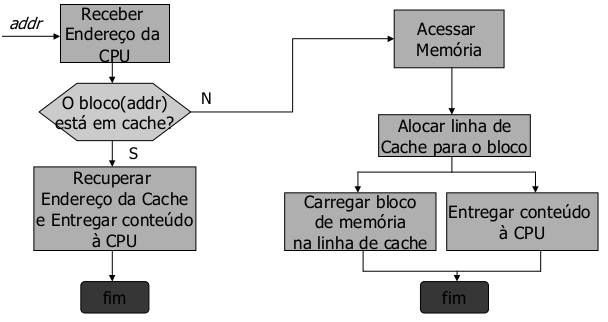
\includegraphics[width=\textwidth]{cache-read}
  \caption{Fluxograma de decisão de leitura da cache}
  \label{fig:reading-cache}
\end{figure}

\subsection{Escrita de Blocos em \textit{Cache}}
Bloco só podem ser alterados/escritos após a confirmação da \textit{tag}, o que torna a operação mais lenta. Além disso, os processadores informam o número de bytes exatos a serem escritos, limitando a operação a essas posições. Na leitura, o acesso à dados a mais não trás problemas.

Temos duas políticas de escrita:
\begin{itemize}
  \item \textbf{Write-through:} dado escrito tanto no bloco em \textit{cache} como na memória. São políticas mais simples e os \textit{read misses} nunca ocasionam escritas para a memória, já que essa política garantem sempre os dados válidos na memória a cada escrita;

  \item \textbf{Write-back:} dado é escrito somente em \textit{cache}. Apenas quando há substituição que o bloco modificado é escrito em memória. Acabam por ser mais rápidas, pois ocorrem só na velocidade de \textit{cache} e usam menos largura de banda já que envia nada a memória.
\end{itemize}

\textsc{Definição} \textbf{Dirty bits:} indicam se o bloco foi modificação enquanto estava em \textit{cache} (\textit{dirty}) ou não (\textit{clean}), sendo que estes últimos não são escritos em memória na substituição.

\textsc{Definição} \textbf{Write Stalls:} ocorrem quando a CPU tem que esperar que o dado seja escrito em memória. Para reduzir este tempo, são usada \textbf{write-buffers}, onde a CPU escreve o dado e continua suas tarefas. O dado então é enviado de maneira assíncrona para a memória.

Em um \textbf{write miss}, o dado antigo não é mais necessário e logo temos duas abordagens para tal:
\begin{itemize}
  \item \textbf{Write allocate:} o bloco é carregado em \textit{cache} no momento do \textit{write miss} e logo depois o \textit{write hit} ocorre;

  \item \textbf{No-write allocate:} o bloco é modificado em memória e não é carregado em \textit{cache}.
\end{itemize}

Políticas \textit{write-back} tendem a usar o primeiro e \textit{write-through} o segundo.

\subsection{Medidas de Desempenho}
Calculamos o tempo média de acesso à memória:
\begin{equation}
  A = T + M * P
\end{equation}

onde $A$ pode ser medido em frações de segundo ou ciclos de clock e:

\begin{itemize}
  \item \textbf{Hit time - $T$:} tempo gasto em um \textit{hit} em cache;
  \item \textbf{Miss rate - $M$:} taxa de misses na cache;
  \item \textbf{Miss penalty - $P$:} penalidade associada a cada miss.
\end{itemize}






\section{Melhoria de Desempenho de Cache}
As caches foram introduzidas para reduzir o gap entre os tempos de aceso à memória principal e a velocidade do processador. O ideal de um projeto de cache seria obter hits rápidos e poucos misses. Logo, temos que melhorar o desempenho dessas caches.

Em se tratando de \textbf{tipos de cache misses}, tempos três tipos, onde eles são relacionados no gráfico da Figura \ref{fig:misses-by-access}:

\begin{itemize}
  \item \textbf{Compulsórios:} no primeiro acesso ao bloco, o mesmo não estará na cache e logo deverá ser trazido para a memória. Também chamados de \textit{cold misses} ou \textit{reference misses};

  \item \textbf{Capacidade:} ocorrem quando um bloco escolhido para substituição é acessado novamente;

  \item \textbf{Conflito:} ocorrem em caches com mapeamento direto ou associativas, se muitos dos blocos referenciados são mapeados para o mesmo conjunto. Também chamados de \textit{collision misses} ou \textit{interference misses}.
\end{itemize}

\begin{figure}[ht]
  \centering
  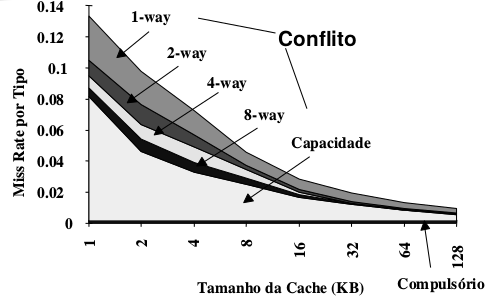
\includegraphics[width=0.8\textwidth]{misses-by-access}
  \caption{Taxas de \textit{misses} por tipo de acesso em um SPEC92, por Patterson}
  \label{fig:misses-by-access}
\end{figure}

\subsection{Reduzindo Cache Misses}

\subsubsection{Aumentar o Tamanho do Bloco}
Quanto maior o tamanho do bloco, menor o número de misses compulsórios, baseando-se no princípio de localidade temporal. Porém, blocos grandes fazem aumentar o número de misses de conflito e capacidade e aumentam a penalidade do miss.
% TODO: não seria espacial??

A escolha do tamanho do bloco leva em conta a latência (tempo de acesso) à memória e a largura de banda à mesma. Em geral, se a largura de banda e a latência são grandes, blocos grandes são escolhidos.

\begin{figure}[ht]
  \centering
  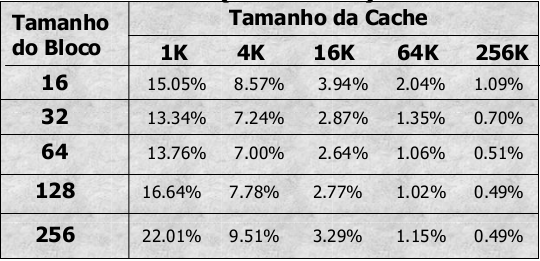
\includegraphics[width=0.8\textwidth]{miss-rate}
  \label{fig:miss-rate}
  \caption{Proporção de \textit{miss rate} ao balancear tamanho de bloco e tamanho de cache}
\end{figure}


\subsubsection{Aumentar a Associatividade}
A justificativa desta técnica é que com maior associatividade, há mais blocos que potencialmente podem ser escolhidos para substituição, possibilitando o uso de algoritmos mais elaborados.

Para utilizar essa técnica, deve-se observar duas regras gerais, obtidas empiricamente:
\begin{itemize}
  \item Uma cache 8-way set associative reduz a taxa de misses tanto quanto uma cache totalmente associativa.

  \item Uma cache de mapeamento direto de tamanho $N$ apresenta aproximadamente o mesmo miss rate que uma cache 2-way associativa de tamanho $\frac{N}{2}$.
\end{itemize}

Logo, devemos ter em mente que, ao aumentar a associatividade, o projeto da cache fica mais complexo e, portanto, o tempo de hit aumenta. Logo, tem de ser pesar as duas grandezas, pois é capaz do tempo médio aumentar.


\subsubsection{Caches Vítimas}
A cache vítima é uma pequena cache totalmente associativa que é adicionada entre a cache e o nível inferior de memória imediatamente inferior. A cache vítima contém somente blocos que foram substituídos da cache por causa de um miss.

Na ocorrência de um misss, verifica-se se o bloco encontra-se na cache vítima. Se sim, o bloco vítima substitui um bloco da cache. Alguns estuso mostram que caches vítimas de poucos bloco (4 em geral) conseguem reduzir o número de misses de conflito de caches pequenas de mapeamento direto.



\subsubsection{Caches Pseudo-Associativas}
Também chamadas de associativas por coluna, essas caches tentam obter a taxa de misses da cache associativa e o tempo de hit da cache de mapeamento direto.

No caso de hit, o acesso a esta cache funciona como o de um mapeamento direto. Em caso de miss, o pseudo-set é obtido pela inversão dos bits mais significativos do índice e a entrada da cache obtida desta maneira é verificada.

Elas possuem um tempo de hit rápido e um tempo de hit lento. Como tal tempo é variável, isso pode complicar o projeto do pipeline. Logo, ela é mais adequada em caches de segundo nível.



\subsubsection{Pré-carga por Hardware de Instrução e Dados}
Intuitivamente, a taxa de misses pode se reduzida se trouxermos os dados e instruções para cache antes dos mesmos terem sido referenciados. É uma ténica comum trazer dois blocos a cada miss: o bloco referenciado e o próximo (localidade espacial). O bloco referenciado é colocado na cache o próximo em um \textit{stream buffer}.



\subsubsection{Pré-carga com Auxílio do Compilador}
Aqui, o compilador insere instruções de pré-carga no código do programa. Em geral, garantimos que o dado ou instrução pré-carregados não causarão excessões de memória virtual (reais ou de proteção). Por esta razão, as pré-cargas mais efetivas são as que não causam alteração no programa (\textit{non-binding prefetching}).

A pré-carga só faz sentido se o processador puder continuar a operação enquanto o dado a ser pré-carregado não chega. Note que as caches devem ser capazes de tratar diversas requisições sem se bloquear (\textit{lockup-free caches}).

A execução de instruções de pré-carga adiciona um overhead à execução, logo é necessário certificar que ele não irá aumentar o tempo geral.



\subsubsection{Otimizações do Compilador}
Técnicas em código, sem usar hardware adicional. Podem ser usadas técnicas de profiling para rearrumar o código, reduzindo misses das instruções.

\textsc{Merging de Arrays}\\
Ao referenciar \textit{arrays} com o mesmo índice no mesmo \textit{loop}, acabamos por gerar misses de conflito, já que as posições dos arrays podem estar em blocos diferentes.

\begin{figure*}[ht]
  \begin{subfigure}[t]{.5\textwidth}
    \centering
    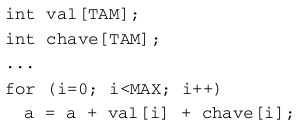
\includegraphics[width=\textwidth]{array-merge-1}
    \caption{\textbf{Código original:} dois \textit{arrays} logicamente conectados, sendo percorridos. Aqui a cada acesso distindo à \texttt{chave{[i]}} e \texttt{valor{[i]}}, podemos ter troca de bloco no cache}
  \end{subfigure}
  ~
  \begin{subfigure}[t]{.5\textwidth}
    \centering
    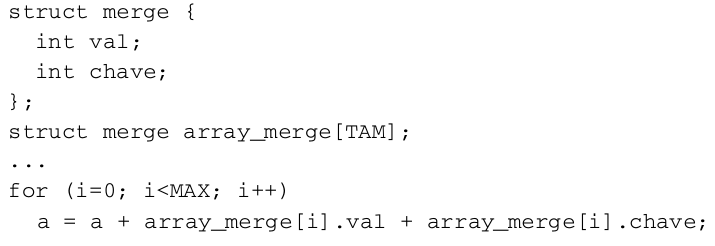
\includegraphics[width=\textwidth]{array-merge-2}
    \caption{\textbf{Código arrumado:} Agora os dados estão sob uma mesma \textit{struct}, logo estão adjacentes na memória. Ganho na localidade espacial quando o bloco for carregado.}
  \end{subfigure}

  \caption{Exemplo de reestruturação de código para \textit{array merge}}
  \label{figs:array-merge}
\end{figure*}




\textsc{Troca de Loops}\\
Loops aninhados que não acessam dados de maneira sequencial podem acabar por acessar bloco diferentes a cada alternância entre as posições. Acesso à matrizes é um bom exemplo. O compilador pode alterar o código de maneira que o acesso seja sequencial.

\begin{figure*}[ht]
  \begin{subfigure}[t]{.5\textwidth}
    \centering
    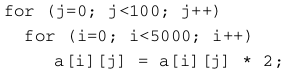
\includegraphics[width=\textwidth]{loop-exchange-1}
    \caption{\textbf{Código original:} exemplo de acesso não sequencial, onde se itera por linha na matriz}
  \end{subfigure}
  ~
  \begin{subfigure}[t]{.5\textwidth}
    \centering
    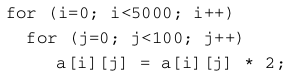
\includegraphics[width=\textwidth]{loop-exchange-2}
    \caption{\textbf{Código arrumado:} agora iteramos por coluna, aproveitando a localidade espacial}
  \end{subfigure}

  \caption{Exemplo de reestruturação de código para troca de \textit{loops}}
  \label{figs:loop-exchange}
\end{figure*}



\textsc{Junção de Loops}\\
O acesso a matrizes com os mesmo loops porém fazendo cálculos diferentes. Logo, podemos tirar proveito da localidade temporal, fazendo que os dados sejam acessados diversas vezes enquanto então em cache.

\begin{figure*}[ht]
  \begin{subfigure}[t]{.5\textwidth}
    \centering
    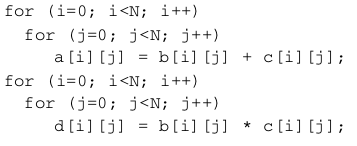
\includegraphics[width=\textwidth]{loop-merge-1}
    \caption{\textbf{Código original:} dois loops iterando sobre a mesma matriz, mas fazendo operações diferentes}
  \end{subfigure}
  ~
  \begin{subfigure}[t]{.5\textwidth}
    \centering
    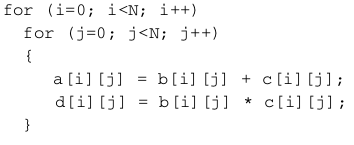
\includegraphics[width=\textwidth]{loop-merge-2}
    \caption{\textbf{Código arrumado:} junção dos dois loops originais em um só. Tiramos proveito da localidade temporal para os dois loops, dado que os dados já estarão em cache}
  \end{subfigure}

  \caption{Exemplo de reestruturação de código para junção de \textit{loops}}
  \label{figs:loop-merge}
\end{figure*}





\textsc{Blocagem}\\
As vezes, quando diversas matrizes são acessas sendo umas por linhas e outras por colunas, podemos realizar uma otimização mais complexa. Operamos em submatrizes (ou blocos), ao invś de se operar sobre a matriz inteira.

\begin{figure*}[ht]
  \begin{subfigure}[t]{.5\textwidth}
    \centering
    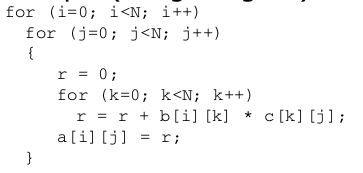
\includegraphics[width=\textwidth]{blocking-1}
    \caption{\textbf{Código original:} \texttt{a} e \texttt{b} percorrem por linha, enquanto \texttt{c} percorre por coluna. Percorremos a matriz inteira sequencialmente.}
  \end{subfigure}
  ~
  \begin{subfigure}[t]{.5\textwidth}
    \centering
    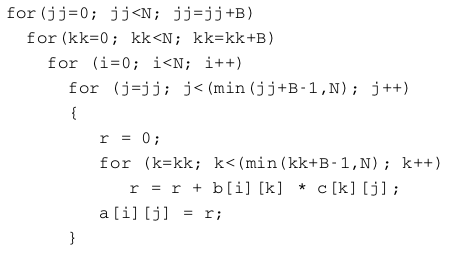
\includegraphics[width=\textwidth]{blocking-2}
    \caption{\textbf{Código arrumado:} criação de submatrizes e percorrimento dessas}
  \end{subfigure}

  \caption{Exemplo de reestruturação de código com blocagem}
  \label{figs:blocking}
\end{figure*}




\subsection{Reduzindo Penalidade do Miss}

\subsubsection{Priorizar Misses de Leitura}
Para acelerar a conclusão da execução de instruções, geralmente \textit{write buffers} são adicionados ao hardware. Logo, quando o store termina, geralmente o dado se encontra neste buffer e não no bloco de cache associado.

Esta decisão pode fazer com que dependendo da ordem de acesso aos dados, valores antigos sejam lidos.

\underline{Exemplo:}

\texttt{1. LOAD 512, r3}\\
\texttt{2. LOAD r1, 1024}\\
\texttt{3. LOAD r2, 512} \\

Caso os endereços 512 e 2014 estejam mapeados no mesmo índice de cache e a escrita de (1) demorar a se completar, a instrução 3 pode ler o valor antigo da memória, havendo um hazard RAW de dados.

A maneira mais simples de evitar que este problema aconteça, consiste em fazer com que o read miss espere até que o \textit{write buffer} esteja vazio. Mas isso aumenta a penalidade do read miss.

Para priorizar misses de leitura, o hardware de muitos processadores verificam o contéudo do \textit{write buffer} e, caso não haja conflito, deixa o read miss continuar.



\subsubsection{Utilizar Sub-blocos}
Consiste em dividir cada bloco da cache em sub-blocos e adicionar um bit de validade a cada sub-bloco. O tag continua associado ao bloco.

Em um read miss, somente um sub-bloco é lido da memória e assim temos a redução da penalidade (menos dados).

\begin{figure}[ht]
  \centering
  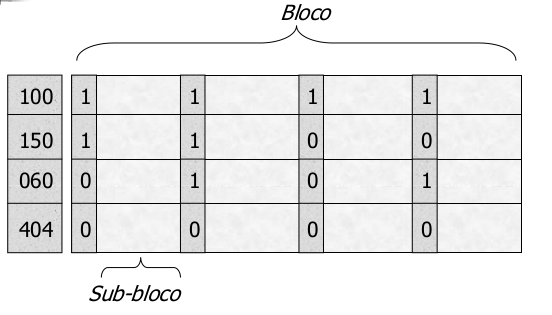
\includegraphics[width=0.8\textwidth]{sub-blocks}
  \label{fig:sub-blocks}
  \caption{Esquema de representação de sub-blocos}
\end{figure}



\subsubsection{Early Restart e Palavra Crítica Primeiro}
Estas técnias não esperam que o bloco inteiro seja colocado em cache, deixando a CPU continuar logo que a palavra desejada esiver carregada.

\begin{itemize}
  \item \textbf{Early restart:} carrega as palavras na ordem sequencial e, logo que a palavra desejada tiver sido carregada, a CPU continuaa a execução.

  \item \textbf{Palavra crítica primeiro:} solicita a palavra que causou o miss primeiro e permite que a CPU continue a execução logo que a mesma chegar
\end{itemize}



\subsubsection{Lockup-free Caches}
Também chamada de \textit{non-blocking cache}, ela é capaz de fornecer dados que estãao na cache mesmo durante um cache miss (\textit{hit under miss}). As mais complexas permitem o tratamento simultâneo de vários misses (\textit{miss under miss}), se a memória for capaz de tratar diversos misses.

O projeto dessas caches é bem complexo, já que lida com diversos acessos incompletos.



\subsubsection{Caches de Segundo Nível}
Como a diferença de desempenho entre RAM e CPU é grande, a inclusão de uma cache mais lentar e de maior capacidade entre a cache tradicional e a memória é interessante. Para serem efetivas, as caches de segundo nível (L2) devem ser bem maiores que a de primeiro nível (L1).

Geralmente, a propriedade de inclusão multinível é observada porém, caso se opte por tamanhos de blocos distintos, o projeto da hierarquia de memória fica complexo.






\subsection{Reduzindo Tempo de Hit}
Esta técnica é interessante uma vez que limita a taxa de clock do processador.


\subsubsection{Caches Simples e Pequenas}
% TODO: ver se está faltando




\subsubsection{Virtual Caches}
Geralmente, a CPU lida com endereços virtuais que devem ser convertidos para endereços físicos e as caches tradicionais utilizam endereços físicos. As caches virtuais utilizam endereços virtuais, não fazendo a tradução de endereços em um cache hit.

No entanto, a cada troca de contexto, a cache deve ser esvaziada (\textit{flushed}), pois cada processo possui seu próprio espaço de endereçamento virtual.



\subsubsection{Pipelining de Escritas}
O pipelining de escritas ocorre entre escritas distintas. Para que o dado seja escrito, primeiramente deve ser feta uma comparação com a tag e depois a escrita é feita no bloco correto. A comparação com a tag é eita no estágio 1 e a escrita no estágio 2.








\section{Memória RAM}
\textsc{Definição} memória semicondutora volátil, onde há a necessidade de um fornecimento constante de energia para manter os valores.

\subsection{DRAM}
Composta por células que armazenam dados, onde um transistor é utilizado para armazenar um bit. É organizada como uma matriz retangular, endereçada por linhas e colunas.

O endereço é dividido em duas metades: \textit{row access strobe} (RAS) e \textit{column access strobe} (CAS). O protocolo de acesso à essa memória é assíncrono. A Figura \ref{fig:dram} mostra o esquema.

\begin{figure}[ht]
  \centering
  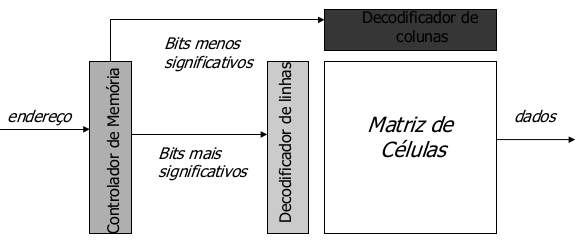
\includegraphics[width=.75\textwidth]{dram}
  \caption{Esquema de acesso à memória DRAM}
  \label{fig:dram}
\end{figure}

As leituras podem danificar o dado contido na célula. Por isso, as DRAMs necessitam de refreshes periódicos para mantê-los. Todos os bits de uma linha podem ser atualizados pela leitura desta linha. Quando há o \textit{refresh}, a memória fica indisponível, um \textit{overhead} que explica o porquê ela é usada mais em memóriais principais.

Para melhorar o desempenho dessas memórias, foca-se em aumentar sua largura de banda. Temos três frentes.

\textsc{Aumento de Tamanho da Palavra}\\
Aumentamos a largura de banda do barramento e logo, transferimos mais dados. Como o acesso da CPU ainda é de uma palavra, é necessário que haja um multiplexador entre a CPU e a \textit{cache}.

\underline{Exemplo:} o Alpha AXP usa barramentos de 256 bits para transferências entre memória RAM e \textit{cache} L2.


\textsc{Memória Entrelaçada}\\
Os chips de memória podem ser organizados em bancos, permitindo que diversas palavras sejam lidas e escritas simultaneamente. Um único controlador de memória é utilizado para isso.

Uma boa função de mapeamento dos endereços para os bancos é crucial para o bom desempenho desta estratégia. A função de módulo normalmente é utilizada,o que favorece acessos sequenciais.

\begin{figure}[ht]
  \centering
  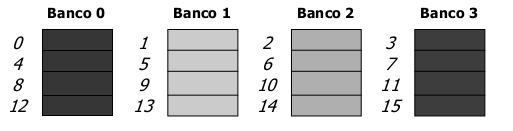
\includegraphics[width=.6\textwidth]{4way-ram}
  \caption{Memória entrelaçada 4-way}
  \label{fig:fourway-ram}
\end{figure}

\textsc{Bancos Independentes de Memória}\\
Aqui existem múltiplos controladores de memória, que permitem que os bancos operem de maneira independente. Cada banco necessita de linhas de endereço separadas e, frequentemente, de barramentos separados.

\subsection{Variações da DRAM}

\textsc{SDRAM}\\
Utiliza um protocol síncrono para troca de dados com o processador, utilizando um relógio externo. O processador informa o endereço e o dado à SDRAM, a qual responde após um número fixo de ciclos de clock. Durante este período, o processador está liberado para outras tarefas.

\textsc{Rambus DRAM}\\
Utiliza um barramento de alta velocidade para trocas entre CPU e memória. Este barramento possui 18 linhas de dados, onde 16 são para o endereço e 2 para paridade. Possui sinais de clock para fazer transações síncronas no barramento.

\textsc{Static DRAM}\\
Utiliza de 4 a 6 transistores por bit, onde os valores binários são armazenados utilizando configurações de flip-flops. o SRAM não necessita de refreshes periódicos, mas ainda precisa de um fornecimento constante de energia.

SRAMs são mais rápidas, mais caras e menos densas que as DRAMs e são muito utilizadas em memórias \textit{cache}.
